\subsection{Experimental Setup and Evaluation Metrics}
Two experiments were conducted. Experiment 1 was designed as the primary model benchmark and compared LR, SVM, KNN, RF, XGBoost, and MLP on scaled data \cite{james2021islr,cortes1995svm,cover1967knn,breiman2001rf,chen2016xgboost,hastie2009esl}.. This setting provided a consistent comparison across model classes while ensuring that scale-sensitive methods were not disadvantaged by variable magnitude differences. Experiment 2 was designed as a preprocessing sensitivity analysis. In this experiment, the tree-based models RF and XGBoost were evaluated across raw, winsorized, and scaled versions of the dataset to assess the extent to which predictive performance changed under alternative data preparation strategies. Because winsorization was introduced only for robustness comparison, the scaled benchmark remained the main reference setting for interpretation.

\subsection{Risk Factor Detection Findings}
The multi-angle risk factor analysis identified several variables with consistent relevance to \texttt{DEATH\_EVENT}. The correlation heatmap in Figure~\ref{fig:corr_heatmap} provides an overview of pairwise associations among numeric variables and illustrates that the dataset contains several non-negligible inter-variable relationships rather than a set of fully independent predictors. In particular, ejection fraction and serum creatinine showed meaningful relationships with the outcome-related structure of the dataset, supporting their relevance for subsequent interpretation. At the same time, the heatmap suggests that most predictors are not so strongly correlated as to make their contributions completely redundant, which supports the use of complementary statistical and model-based approaches for factor detection.

\begin{figure}[H]
\centering
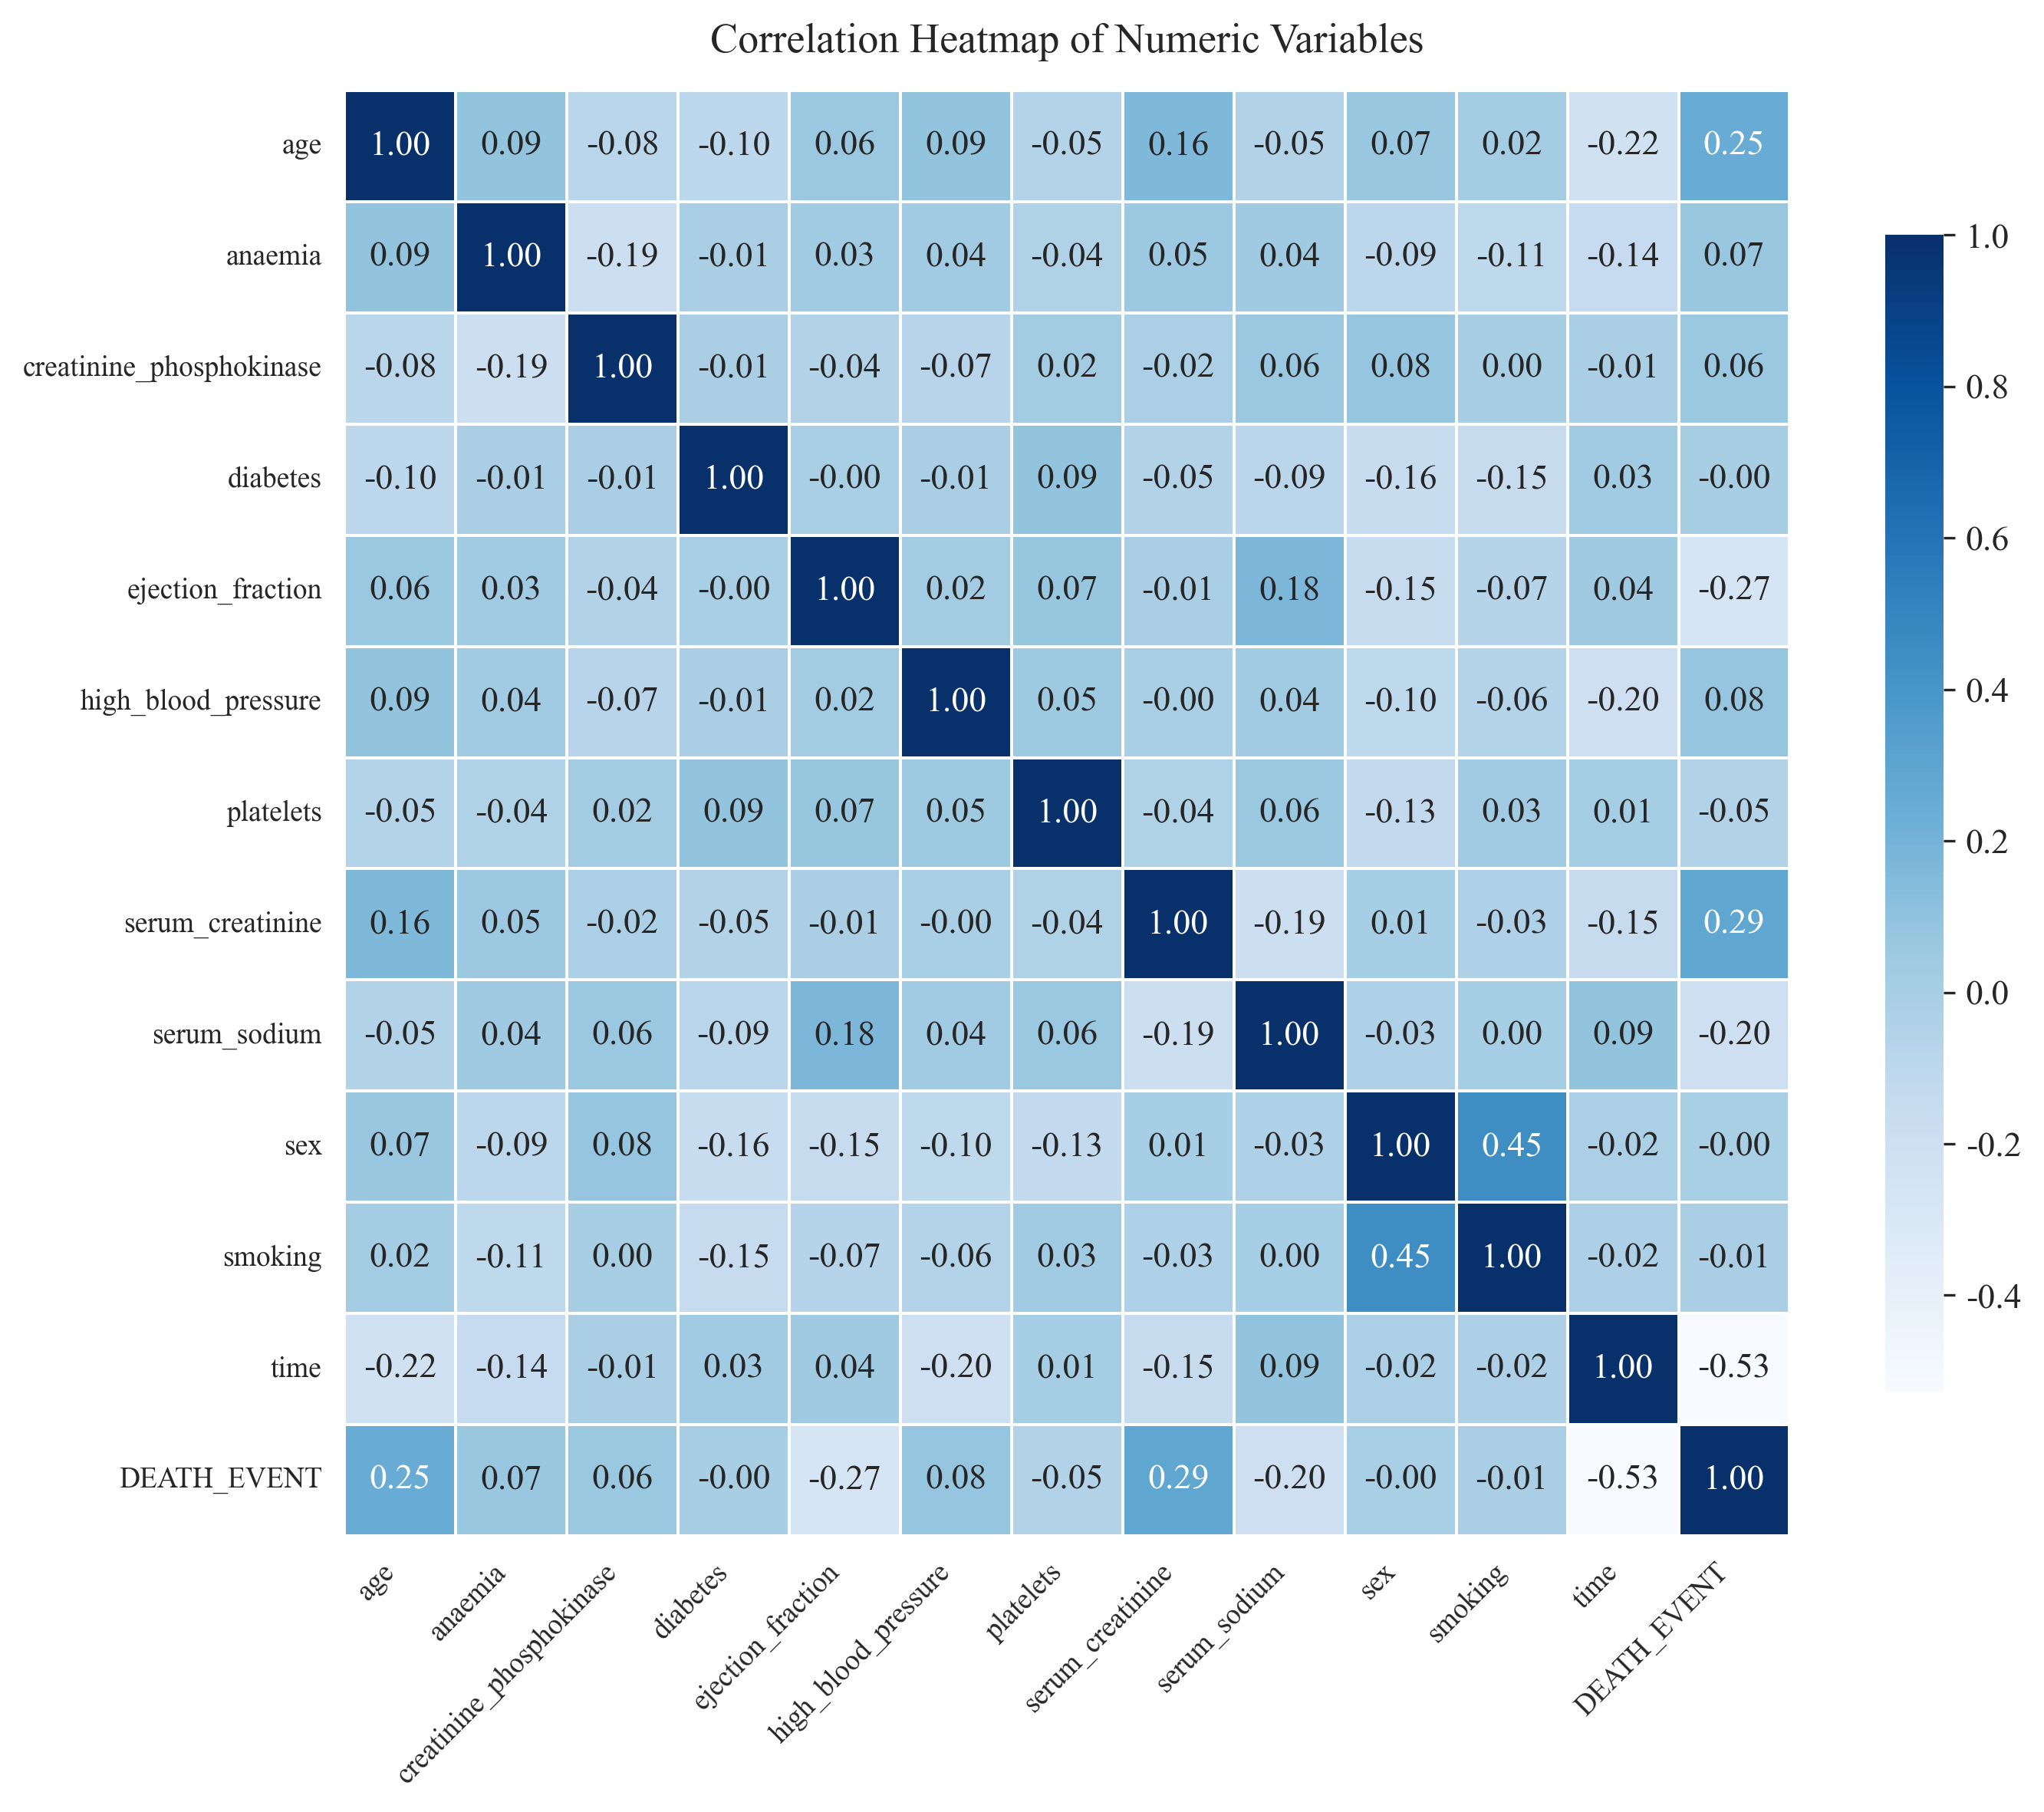
\includegraphics[width=0.7\textwidth]{figures/correlation_heatmap.png}
\caption{Correlation heatmap of numeric variables used in risk factor analysis.}
\label{fig:corr_heatmap}
\end{figure}

In the univariate analysis, follow-up time showed the strongest association with outcome, followed by ejection fraction, age, serum creatinine, and serum sodium. No binary variable reached statistical significance in the chi-square analysis. These findings suggest that the measurable prognostic signal in this dataset is concentrated primarily in continuous clinical and laboratory variables rather than in the assessed binary indicators.


The model-based analysis showed a similar pattern. As shown in Figure~\ref{fig:rf_importance}, random-forest-derived feature importance ranked follow-up time, serum creatinine, ejection fraction, age, and creatinine phosphokinase as the most influential variables. The distribution of importance values indicates that follow-up time contributed substantially more than the remaining predictors, while serum creatinine and ejection fraction formed a second tier of clinically interpretable variables with clear prognostic relevance. Age and creatinine phosphokinase also contributed meaningfully, although with smaller importance values.

When statistical ranking and model importance were considered jointly, follow-up time, ejection fraction, and serum creatinine emerged as the most prominent factors overall. Although follow-up time was highly informative for discrimination, its interpretation remains conditional on dataset structure. Greater clinical emphasis should therefore be placed on variables such as ejection fraction and serum creatinine, which are more directly linked to cardiac function and cardiorenal status.


\begin{figure}[H]
\centering
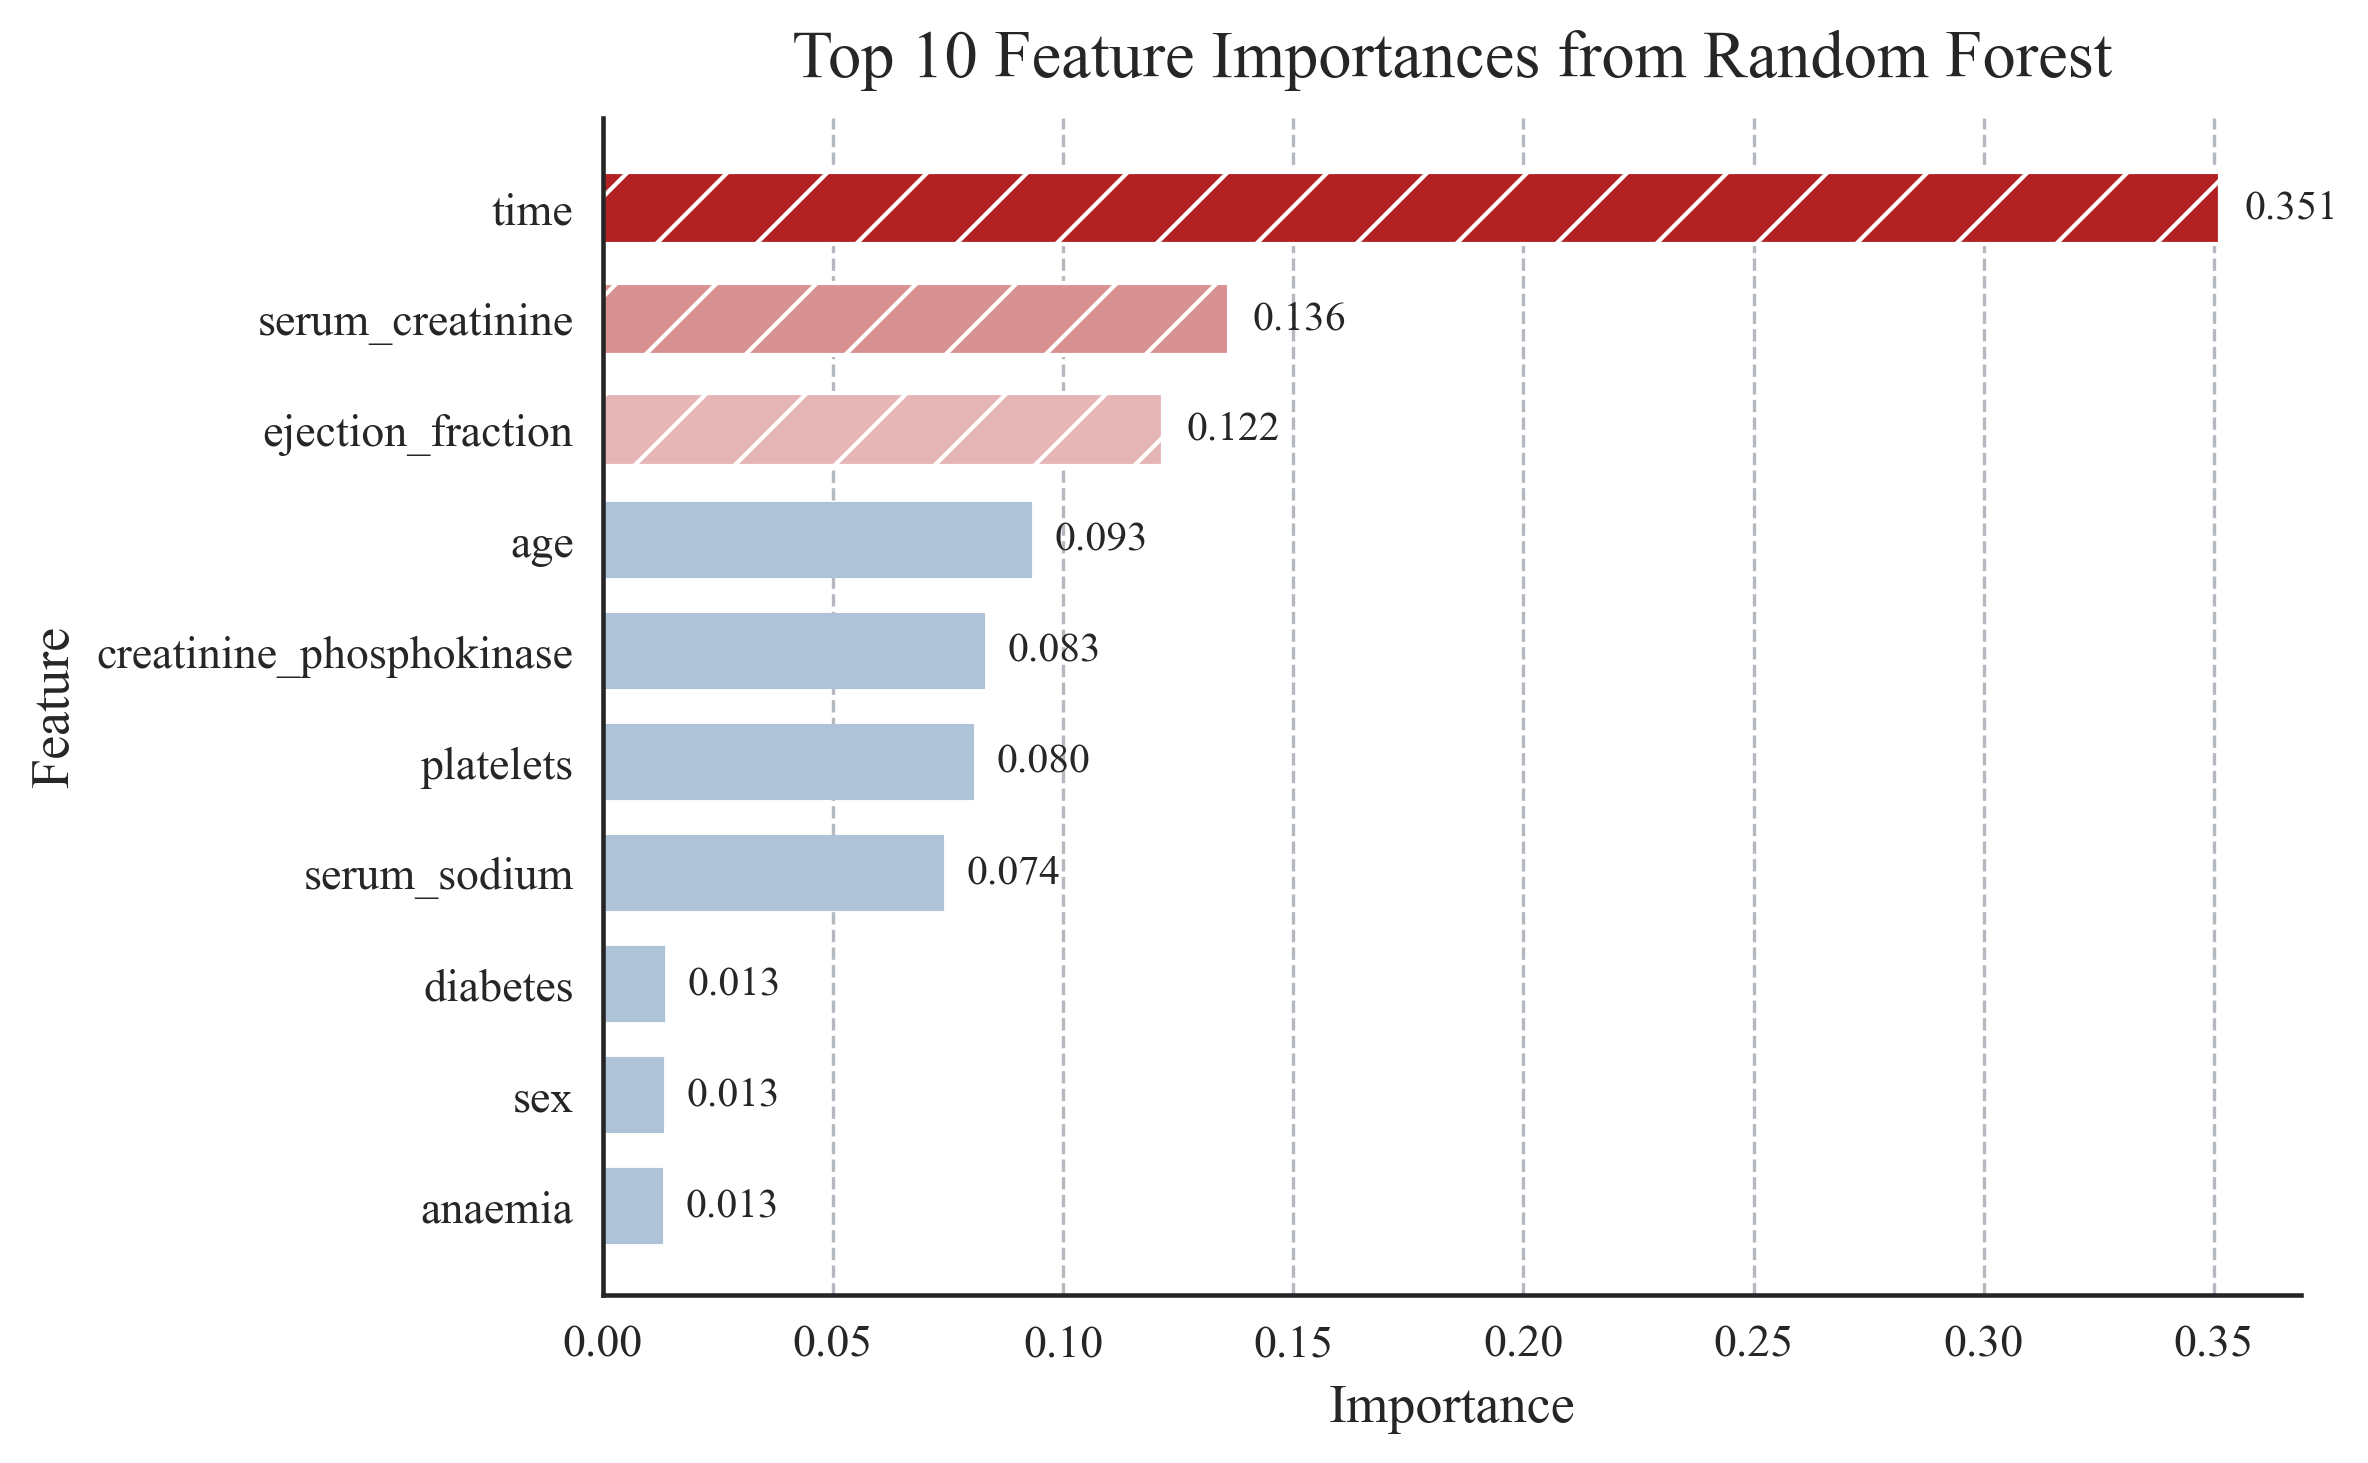
\includegraphics[width=0.76\textwidth]{figures/feature_importance.png}
\caption{Random-forest-derived feature importance ranking for risk factor analysis.}
\label{fig:rf_importance}
\end{figure}

\subsection{Experiment 1: Model Benchmark on Scaled Data}
The primary experiment compared six models on scaled data. The strongest overall performance was observed for the tree-based ensemble methods. XGBoost achieved the highest accuracy (0.8333), precision (0.8462), and F1-score (0.6875), whereas random forest achieved the highest AUC (0.8960) with accuracy 0.8167, precision 0.7857, recall 0.5789, and F1-score 0.6667. Logistic regression also reached accuracy 0.8167 and F1-score 0.6667, but with a lower AUC of 0.8614.

\begin{figure}[H]
\centering
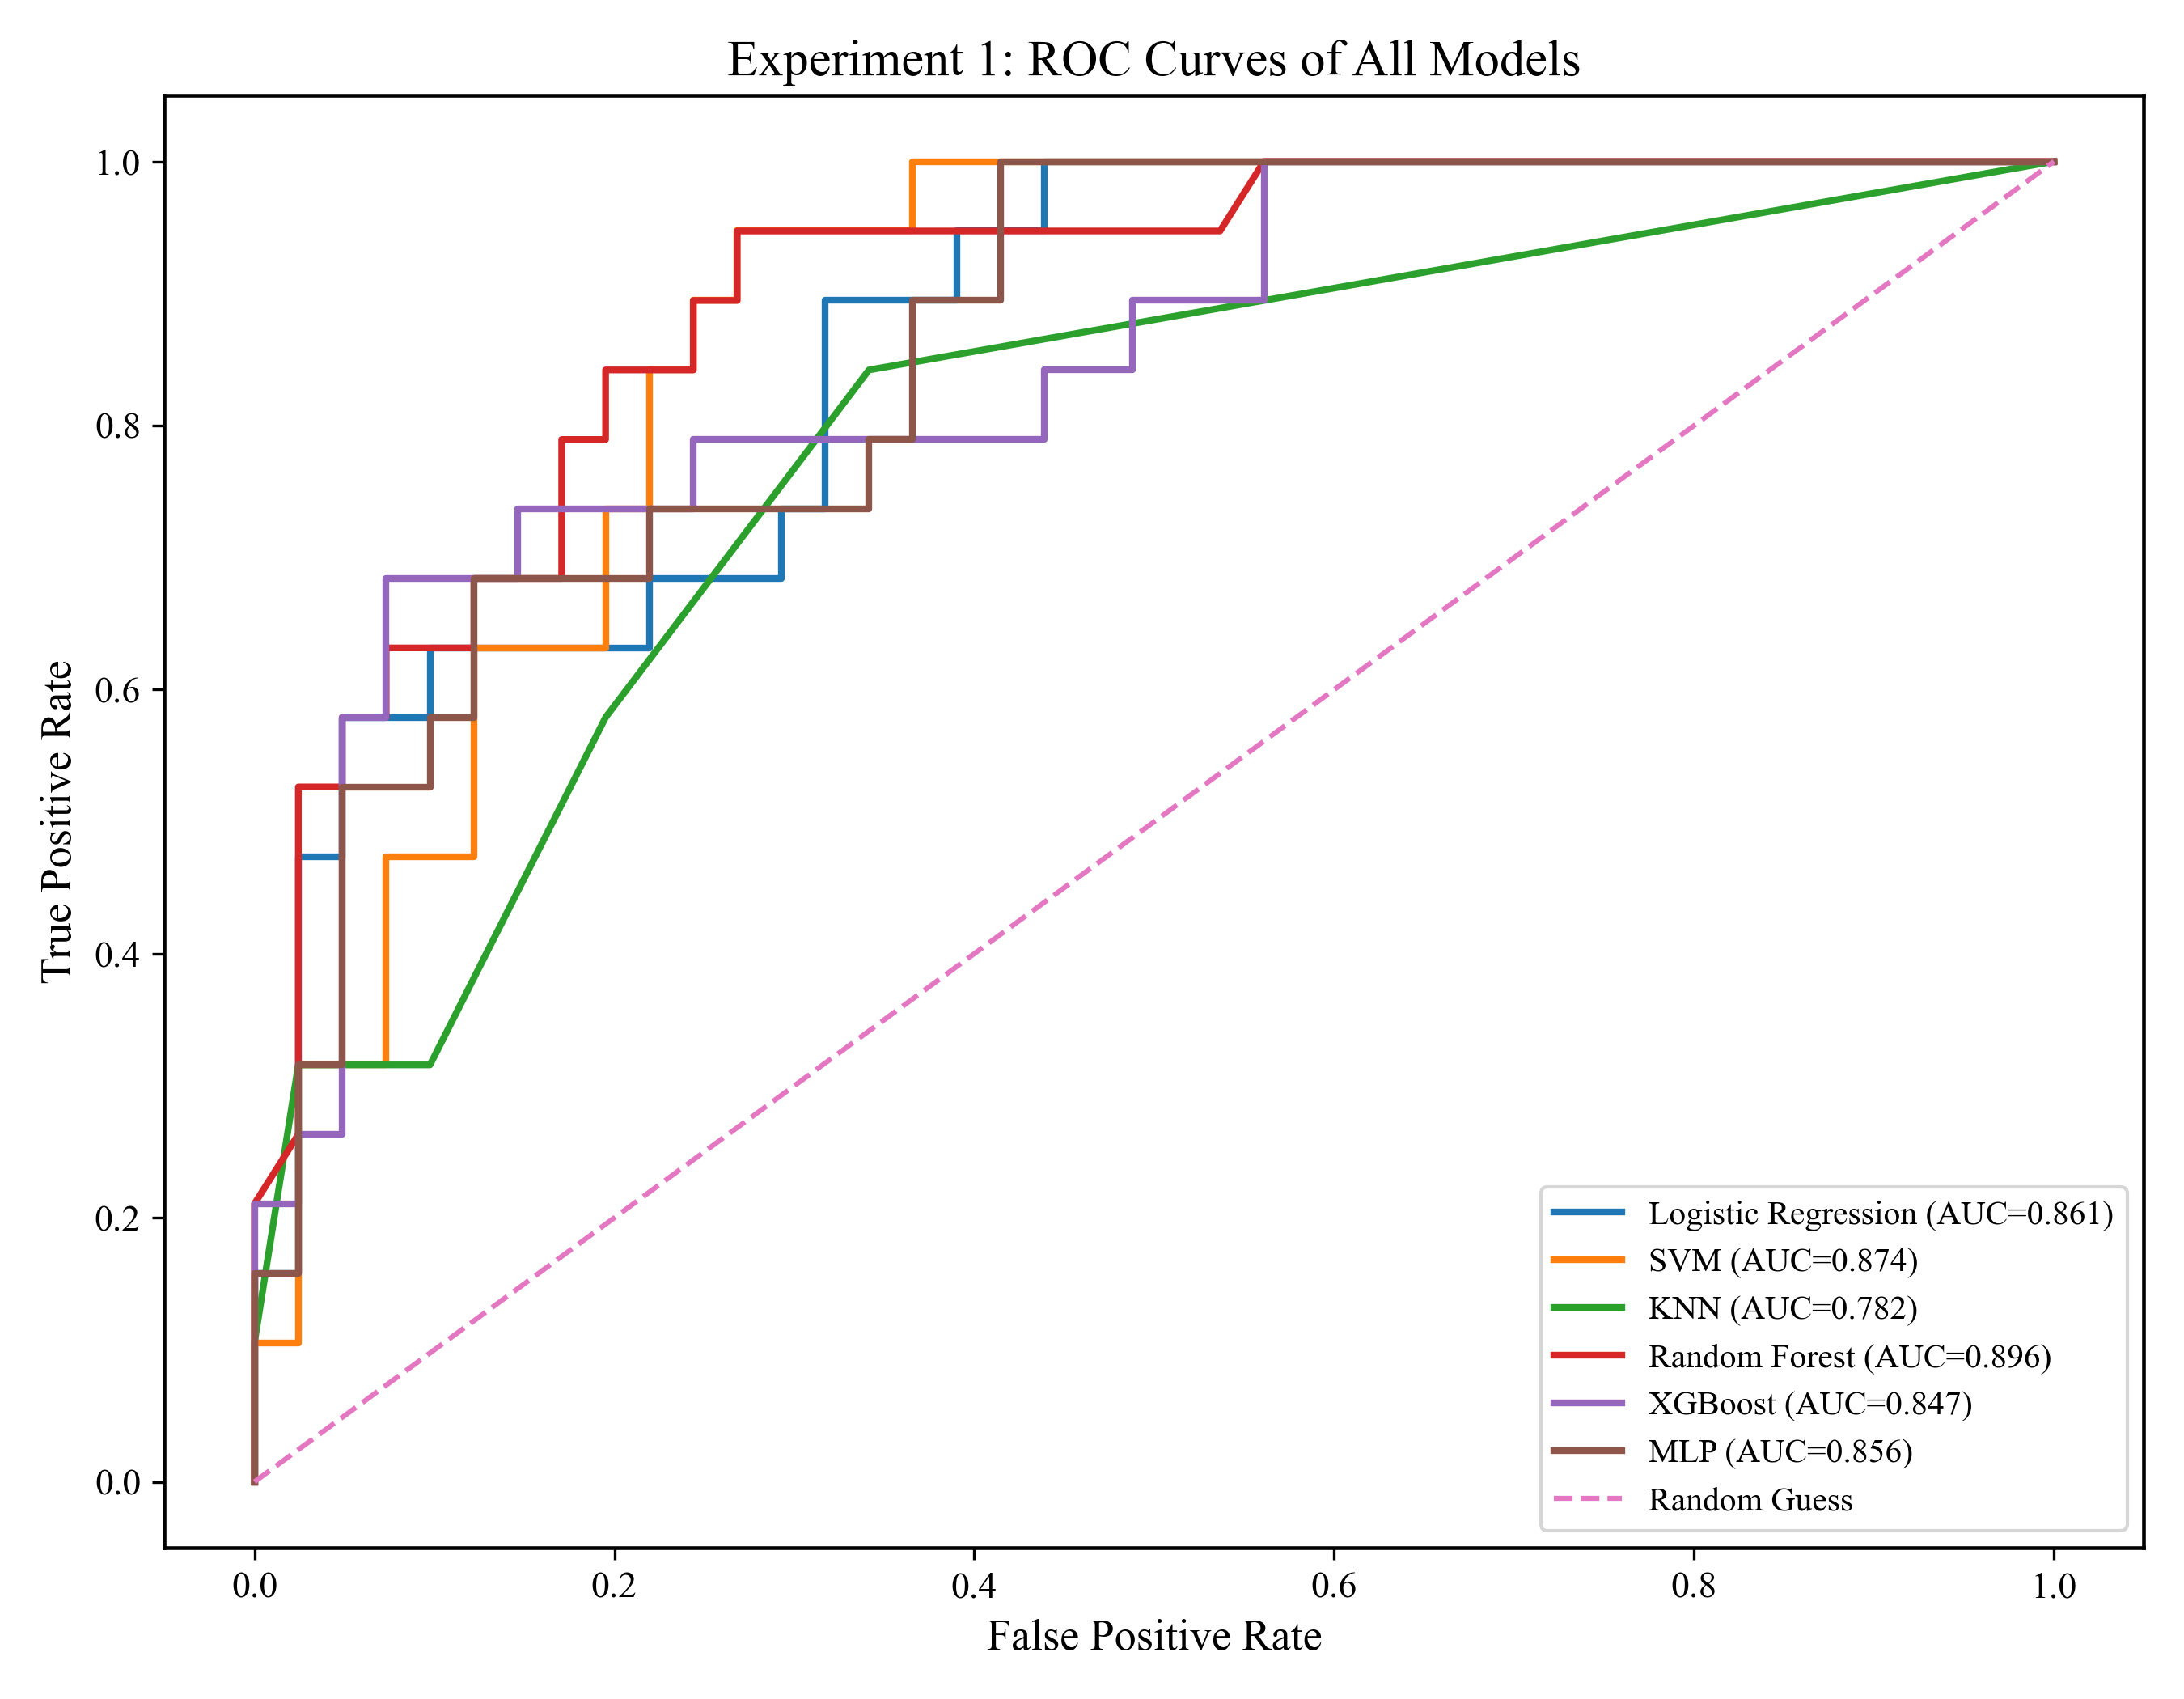
\includegraphics[width=0.76\textwidth]{figures/experiment1_roc.png}
\caption{Receiver operating characteristic curves for Experiment 1 model comparison on scaled data.}
\label{fig:experiment1_roc}
\end{figure}

Among the remaining baselines, SVM achieved accuracy 0.7667, precision 0.6923, recall 0.4737, F1-score 0.5625, and AUC 0.8742. KNN showed the weakest overall results, with accuracy 0.7167, precision 0.6000, recall 0.3158, F1-score 0.4138, and AUC 0.7824. The MLP baseline achieved accuracy 0.8000, precision 0.7333, recall 0.5789, F1-score 0.6471, and AUC 0.8562. Taken together, these results indicate that the two ensemble tree methods produced the most favorable balance between threshold-based classification metrics and discrimination, while the simpler and neural baselines remained competitive but not superior. The ROC curves in Figure~\ref{fig:experiment1_roc} illustrate the relative discrimination achieved by the compared methods.

\subsection{Experiment 2: Preprocessing Sensitivity Analysis}
The secondary experiment examined whether the performance of random forest and XGBoost changed across raw, winsorized, and scaled versions of the data. For random forest, performance varied only modestly across preprocessing settings. Accuracy was 0.8000 on raw data and 0.8167 on both winsorized and scaled data. The corresponding AUC values were 0.8935 for raw data, 0.8864 for winsorized data, and 0.8960 for scaled data. Precision, recall, and F1-score were 0.7692, 0.5263, and 0.6250 on raw data, compared with 0.7857, 0.5789, and 0.6667 on both winsorized and scaled data.


\begin{figure}[H]
\centering
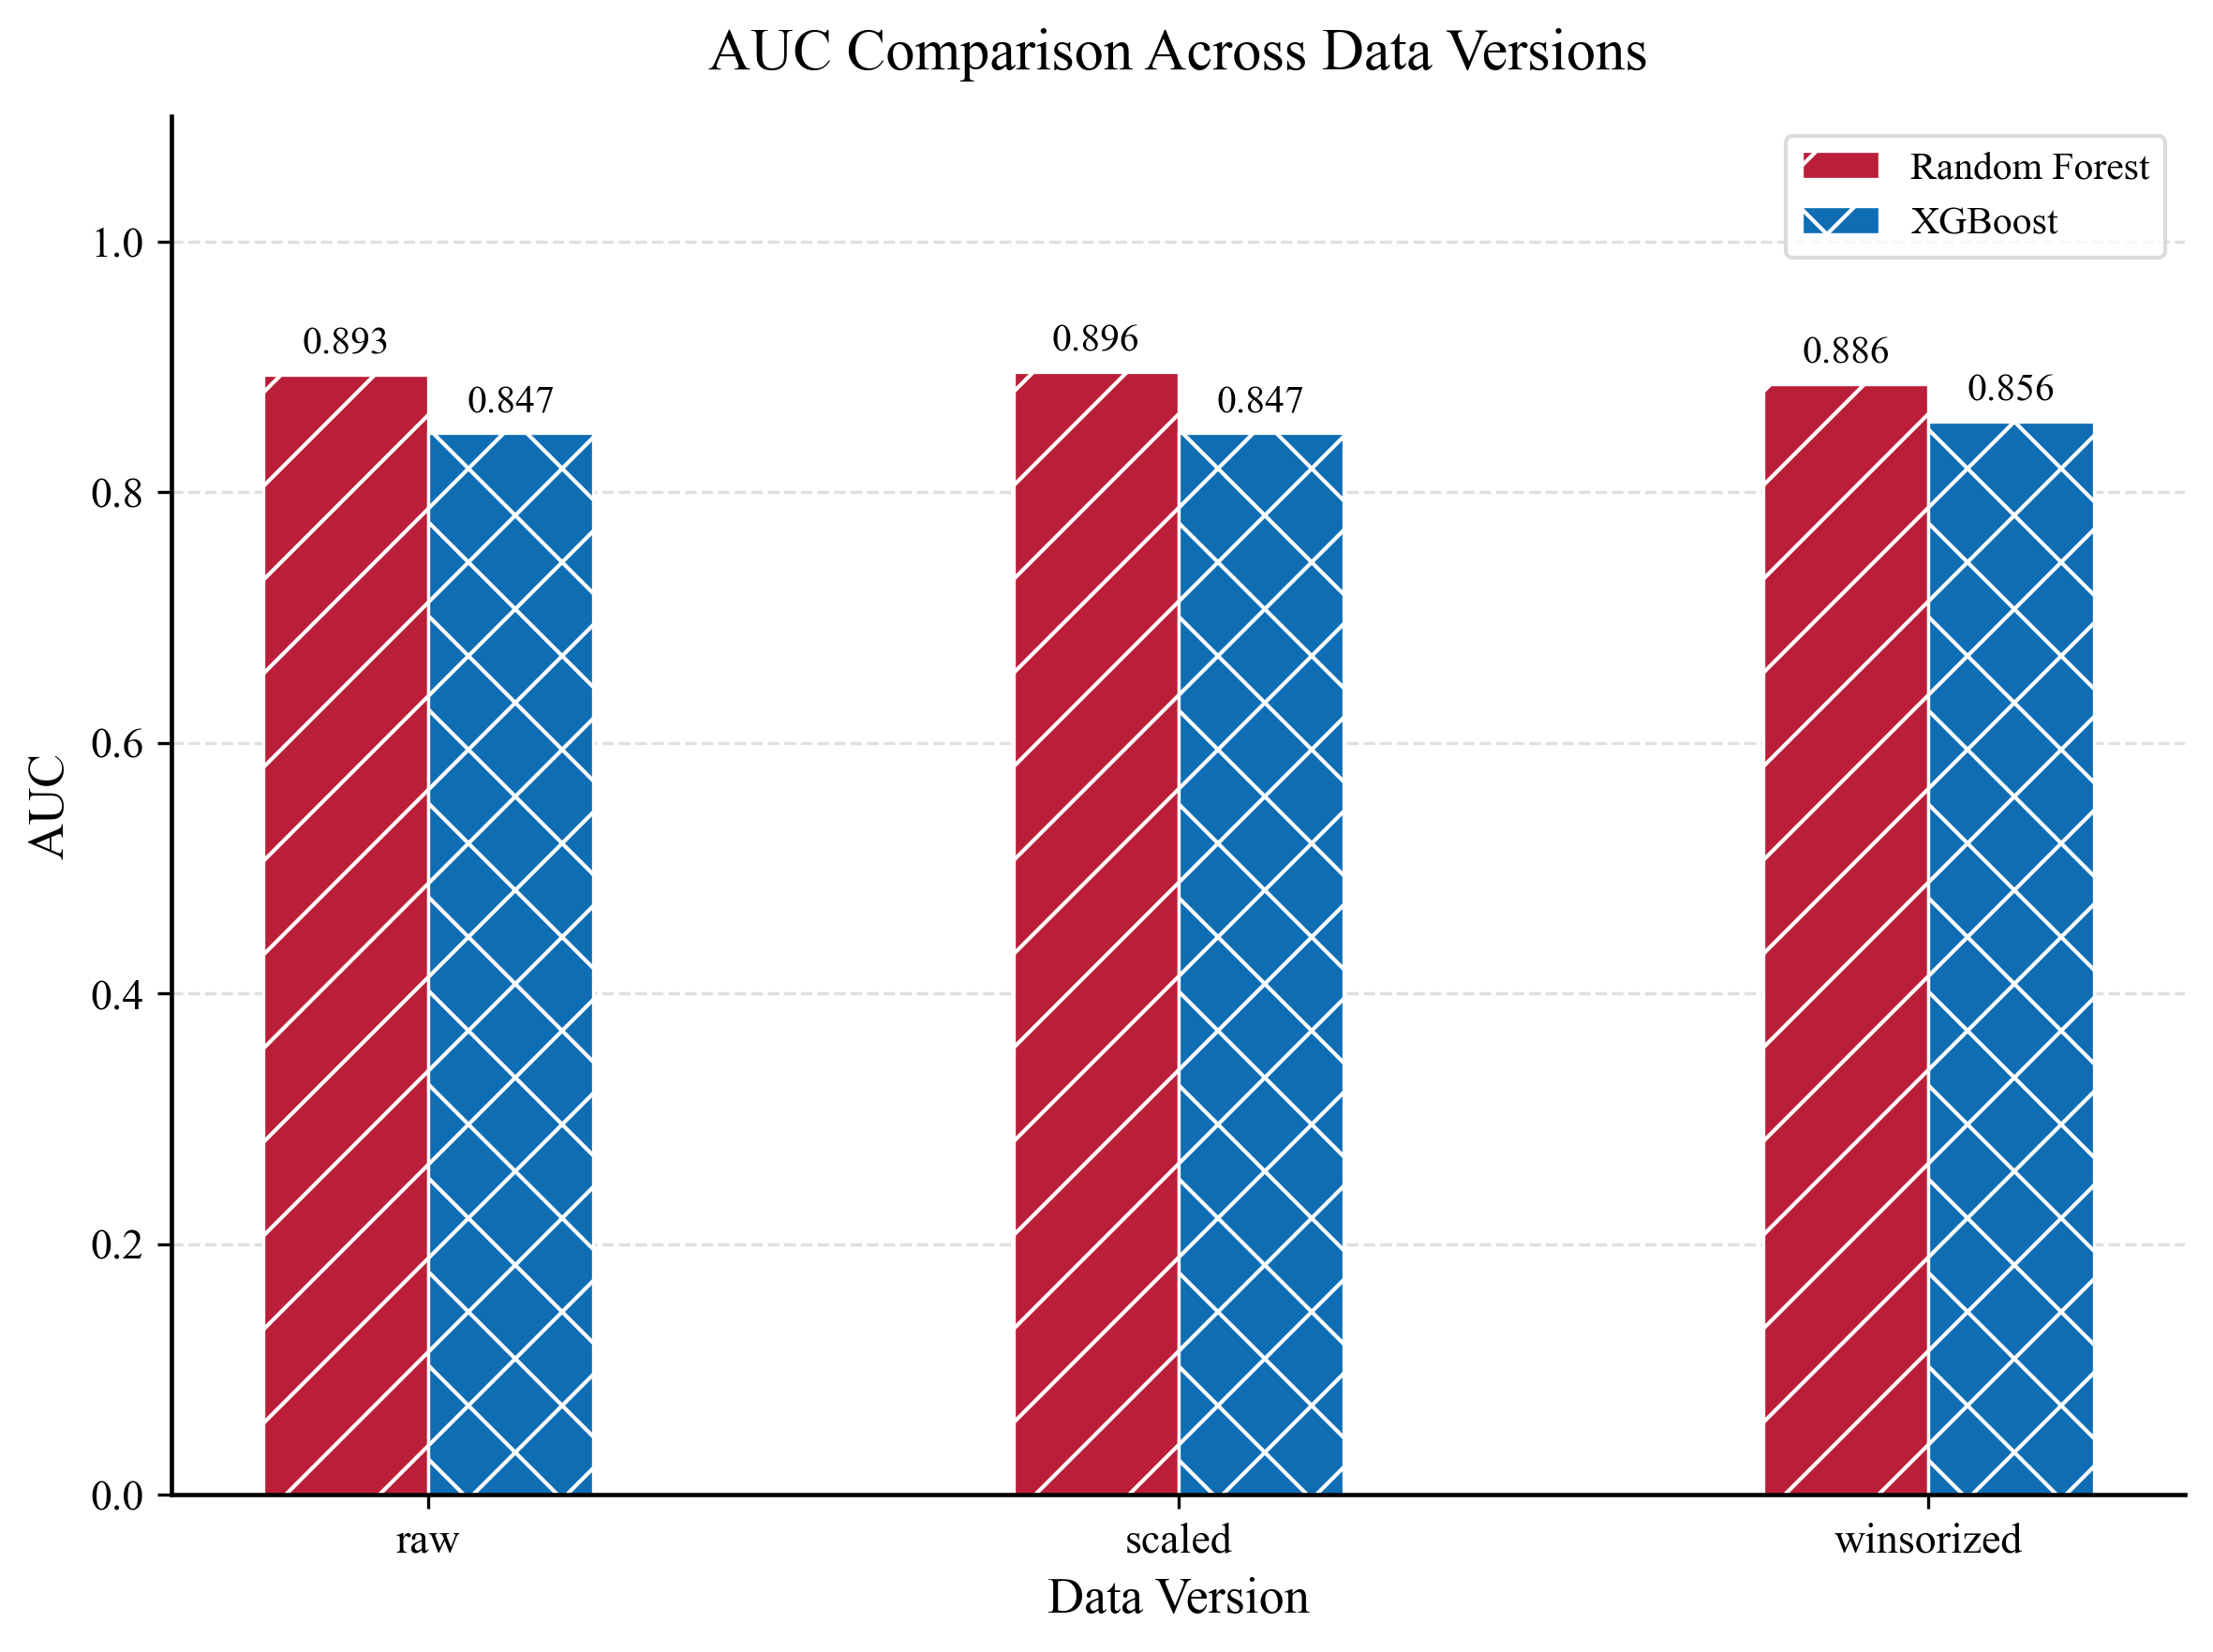
\includegraphics[width=0.6\textwidth]{figures/experiment2_auc_bar.png}
\caption{AUC comparison for random forest and XGBoost across raw, winsorized, and scaled data versions.}
\label{fig:experiment2_auc}
\end{figure}

XGBoost showed similarly stable behavior across preprocessing variants. Accuracy, precision, recall, and F1-score remained unchanged at 0.8333, 0.8462, 0.5789, and 0.6875, respectively, for raw, winsorized, and scaled data. The AUC values were 0.8472 on raw data, 0.8562 on winsorized data, and 0.8472 on scaled data. As shown in Figure~\ref{fig:experiment2_auc}, the overall ranking of preprocessing strategies was similar across the two models, with no large shifts in discriminative performance.

\subsection{Individual Mortality Probability Prediction for a New Patient}
To further illustrate patient-level inference, an example prediction was generated for a new patient using the model with the strongest discriminative performance in the benchmark analysis. For this case, the predicted mortality probability was 0.5567, with a corresponding positive class prediction under the default decision threshold. Although presented here as an application example rather than a separate validation experiment, this result demonstrates that the proposed framework can provide individualized probability estimates in addition to cohort-level comparative performance.

\begin{table}[H]
\centering
\caption{Example of individual mortality probability prediction for a new patient.}
\label{tab:new_patient_prediction}
\resizebox{\textwidth}{!}{
\begin{tabular}{ccccccc}
\toprule
Age & Ejection Fraction & Serum Creatinine & Serum Sodium & Follow-up Time & Predicted Probability & Predicted Class \\
\midrule
68 & 25 & 1.8 & 132 & 90 & 0.5567 & 1 \\
\bottomrule
\end{tabular}
}
\end{table}

In this example, the patient exhibited reduced ejection fraction and elevated serum creatinine, both of which had previously emerged as prominent prognostic variables in the multi-angle factor analysis. The predicted probability is therefore consistent with the broader analytical findings and illustrates how the framework may be used to summarize individualized mortality risk in probabilistic terms.
